% ==========================================================
% ENTREGA 1 — O corpus do projeto
% Projeto Integrador III — Motor de Busca — Ciência de Dados
% Fatec Baixada Santista – Rubens Lara
% Derivado de modelo-trabalho.Rnw (R + knitr + abnTeX2)
% ==========================================================
%
% O QUE ENTREGAR
%   Um texto de NO MÁXIMO 3 PÁGINAS, com quatro seções:
%     1. Introdução ................... o tema, quem o buscaria, o que este texto faz
%     2. A fonte e o documento ........ a escolha do corpus e a motivação dela
%     3. Como o corpus foi obtido ..... os passos da coleta e o que deu errado
%     4. Defesa do corpus ............. a evidência de que ele serve para o motor
%   Mais as Referências (não contam nas 3 páginas).
%
% ONDE ENTREGAR
%   O PDF e este .Rnw em  consolidados/
%   O corpus em  estrutura/banco-de-dados/  (docs.rds, origem.rds); o codigo da coleta em estrutura/codigo/aula01.ipynb
%   A ficha do projeto em  consolidados/00_FICHA_PROJETO.md  — as seções 1 e 2
%   deste texto são a ficha em prosa; as duas têm que dizer a mesma coisa.
%
% COMO COMPILAR
%   RStudio: Tools > Global Options > Sweave >
%            "Weave Rnw files using: knitr" e "Typeset LaTeX into PDF using: pdfLaTeX".
%            Depois, botão "Compile PDF".
%   Terminal: Rscript -e "knitr::knit2pdf('entrega-1-corpus.Rnw')"
%
% ARQUIVOS NECESSÁRIOS NA MESMA PASTA
%   entrega-1-corpus.Rnw   (este arquivo)
%   referencias.bib        (as referências em BibTeX)
%
% REQUISITOS
%   R com knitr; LaTeX com abntex2 (TeX Live: texlive-publishers).
%   Salve em UTF-8. Se acentos saírem como <U+00E9>, a sessão do R não
%   está em locale UTF-8 (Linux: LANG=pt_BR.UTF-8 ou C.UTF-8).
% ==========================================================

\documentclass[
  article,
  12pt,
  oneside,
  a4paper,
  english,
  brazil
]{abntex2}\usepackage[]{graphicx}\usepackage[]{xcolor}
% maxwidth is the original width if it is less than linewidth
% otherwise use linewidth (to make sure the graphics do not exceed the margin)
\makeatletter
\def\maxwidth{ %
  \ifdim\Gin@nat@width>\linewidth
    \linewidth
  \else
    \Gin@nat@width
  \fi
}
\makeatother

\definecolor{fgcolor}{rgb}{0.345, 0.345, 0.345}
\newcommand{\hlnum}[1]{\textcolor[rgb]{0.686,0.059,0.569}{#1}}%
\newcommand{\hlsng}[1]{\textcolor[rgb]{0.192,0.494,0.8}{#1}}%
\newcommand{\hlcom}[1]{\textcolor[rgb]{0.678,0.584,0.686}{\textit{#1}}}%
\newcommand{\hlopt}[1]{\textcolor[rgb]{0,0,0}{#1}}%
\newcommand{\hldef}[1]{\textcolor[rgb]{0.345,0.345,0.345}{#1}}%
\newcommand{\hlkwa}[1]{\textcolor[rgb]{0.161,0.373,0.58}{\textbf{#1}}}%
\newcommand{\hlkwb}[1]{\textcolor[rgb]{0.69,0.353,0.396}{#1}}%
\newcommand{\hlkwc}[1]{\textcolor[rgb]{0.333,0.667,0.333}{#1}}%
\newcommand{\hlkwd}[1]{\textcolor[rgb]{0.737,0.353,0.396}{\textbf{#1}}}%
\let\hlipl\hlkwb

\usepackage{framed}
\makeatletter
\newenvironment{kframe}{%
 \def\at@end@of@kframe{}%
 \ifinner\ifhmode%
  \def\at@end@of@kframe{\end{minipage}}%
  \begin{minipage}{\columnwidth}%
 \fi\fi%
 \def\FrameCommand##1{\hskip\@totalleftmargin \hskip-\fboxsep
 \colorbox{shadecolor}{##1}\hskip-\fboxsep
     % There is no \\@totalrightmargin, so:
     \hskip-\linewidth \hskip-\@totalleftmargin \hskip\columnwidth}%
 \MakeFramed {\advance\hsize-\width
   \@totalleftmargin\z@ \linewidth\hsize
   \@setminipage}}%
 {\par\unskip\endMakeFramed%
 \at@end@of@kframe}
\makeatother

\definecolor{shadecolor}{rgb}{.97, .97, .97}
\definecolor{messagecolor}{rgb}{0, 0, 0}
\definecolor{warningcolor}{rgb}{1, 0, 1}
\definecolor{errorcolor}{rgb}{1, 0, 0}
\newenvironment{knitrout}{}{} % an empty environment to be redefined in TeX

\usepackage{amsmath}
\usepackage{alltt}

\usepackage[T1]{fontenc}
\usepackage[utf8]{inputenc}
\usepackage{lmodern}
\usepackage{amsmath,amssymb}
\usepackage{icomma}
\usepackage{booktabs}
\usepackage{xcolor}
\usepackage[alf]{abntex2cite}

\hypersetup{hidelinks}

% ----------------------------------------------------------
% DADOS DA ENTREGA — preencha aqui
% ----------------------------------------------------------
\titulo{O corpus do projeto: \textit{escreva aqui o tema, em uma linha}}
% O abntex2 imprime um "titulo estrangeiro" logo abaixo do titulo quando o
% documento declara mais de um idioma. Deixe vazio se nao houver.
\tituloestrangeiro{}
\autor{Nome do Grupo}
\local{Santos-SP}
\data{\today}

\newcommand{\nomecurso}{Tecnologia em Ciência de Dados}
\newcommand{\nomedisciplina}{Projeto Integrador III --- Motor de Busca}
\newcommand{\nomeprofessor}{Prof.\ Dr.\ João Paulo Ferreira de Mello}
\newcommand{\repositorio}{projeto-nome-do-grupo}
% Um integrante por linha: Nome Completo -- RA
\newcommand{\integrantes}{%
  Nome Completo do Integrante 1 -- RA 0000000000000 \\
  Nome Completo do Integrante 2 -- RA 0000000000000 \\
  Nome Completo do Integrante 3 -- RA 0000000000000%
}
\IfFileExists{upquote.sty}{\usepackage{upquote}}{}
\begin{document}





\selectlanguage{brazil}
\frenchspacing

% ----------------------------------------------------------
% IDENTIFICAÇÃO
% ----------------------------------------------------------
\maketitle

\begin{center}
  \small
  Fatec Baixada Santista -- Rubens Lara \\
  \nomecurso{} \quad|\quad \nomedisciplina{} \quad|\quad \nomeprofessor{} \\[0.4em]
  \integrantes \\[0.4em]
  Repositório: \texttt{\repositorio}
\end{center}

\begin{center}\color{red}\textbf{ATEN\c{C}\~AO: compilado com o corpus de teste da aula, n\~ao com o do grupo.}\end{center}


\textual

% ==========================================================================
\section{Introdução}
% ==========================================================================
% ~meia página. O QUE VAI AQUI:
%   - o tema do motor de busca, em uma frase, e a ligação com a Baixada
%     Santista (o lugar, a história, a atividade, as pessoas);
%   - quem usaria o motor e o que essa pessoa quer descobrir;
%   - as três perguntas que o motor deve responder (as da ficha, seção 2);
%   - o que este texto entrega: o corpus escolhido, como foi obtido, e a
%     evidência de que ele serve.
% NÃO adiante aqui os números da Seção 4.

Apresente o tema e diga por que ele interessa, e a quem. Em recuperação de
informação, o que se atende é a \emph{necessidade de informação} de alguém, não
a consulta literal \cite[cap.~1]{manning2008}; por isso as perguntas vêm antes
do corpus. Feche o primeiro parágrafo dizendo, em uma frase, o que este texto
faz: apresenta a fonte escolhida, descreve como o corpus foi montado e mostra
que ele tem condição de responder às perguntas.

% ==========================================================================
\section{A fonte e o documento}
% ==========================================================================
% ~três quartos de página. O QUE VAI AQUI:
%   - ORIGEM: de onde veio o texto (Wikipédia, portal, jornal...), com a
%     referência bibliográfica, a LICENÇA e a data de acesso;
%   - AS PÁGINAS: os títulos exatos usados, e por que essas;
%   - O DOCUMENTO: o que é UMA LINHA do corpus (um parágrafo? uma notícia?
%     uma seção?) e por quê -- o critério é "a menor unidade que responde
%     sozinha a uma pergunta";
%   - MOTIVAÇÃO: por que este corpus, e não outro. Responda honestamente:
%     interesse pelo assunto? disponibilidade? conhecimento prévio do
%     grupo? Todas são razões legítimas -- o que não vale é não ter razão.
%     Cite a alternativa que foi descartada, e por quê.

Descreva a origem, com a referência \cite{wikipedia}, a licença e a data de
acesso. Liste as páginas. O corpus tem $N = \text{8}$ documentos vindos
de \text{2} páginas.

Diga o que é um documento e justifique. Um artigo inteiro como documento faz a
busca devolver ``a resposta está no artigo de X'' sem dizer onde; o parágrafo
é o padrão do curso, mas o grupo pode ter decidido outra coisa --- e então
explica.

Explique a escolha do tema e da fonte, e a alternativa descartada.

% ==========================================================================
\section{Como o corpus foi obtido}
% ==========================================================================
% ~meia página. O QUE VAI AQUI:
%   - os passos da coleta (notebook aula01.ipynb), na ordem em que rodam (chamada à API, quebra
%     em parágrafos, filtro, montagem do vetor, gravação) -- em prosa, sem
%     colar código: o código está em estrutura/codigo/aula01.ipynb;
%   - O QUE DEU ERRADO e o que o grupo fez: título de página errado,
%     parágrafos que eram listas ou referências, artigo que dominou o
%     corpus, acentos... Esta parte é obrigatória. Coleta sem problema
%     não existe.

Descreva os passos. O critério de documento foi ``parágrafo com mais de
\text{200} caracteres''; diga como esse número foi escolhido.

Conte o que deu errado e o que mudou por causa disso.

% ==========================================================================
\section{Defesa do corpus}
% ==========================================================================
% ~uma página. É A SEÇÃO QUE PESA MAIS. O QUE VAI AQUI:
%   - o diagnóstico do corpus (Tabela 1 e Tabela 2), comentado item a item;
%   - a passagem pelos quatro descartes: tamanho, domínio de uma página,
%     documentos que não são prosa, sujeira -- dizendo o que foi encontrado
%     e o que o grupo fez a respeito;
%   - a figura dos tamanhos (Figura 1), com uma frase de leitura;
%   - os dez termos mais frequentes: quantos dizem algo sobre o tema?
%   - o veredito: o corpus responde às três perguntas da Introdução?
%     Se um descarte pegou, o que mudou no corpus por causa dele?
% Os números desta seção saem do bloco <<dados>> -- eles se atualizam
% sozinhos quando voces trocarem os .rds.

A Tabela~\ref{tab:diag} reúne as verificações feitas sobre o corpus, e a
Tabela~\ref{tab:origem} mostra de onde veio cada documento.

\begin{table}[htb]
  \centering
  \caption{Diagnóstico do corpus}
  \label{tab:diag}
  \small
  \begin{tabular}{@{}p{0.34\textwidth}p{0.58\textwidth}@{}}
    \toprule
    \textbf{Verificação} & \textbf{Resultado} \\
    \midrule
    Tamanho ($N$ documentos, páginas) & $\text{8}$ documentos de $\text{2}$ páginas \\
    Tokens por documento              & 6 a 9 (m\'edia 8) \\
    Vocabulário bruto                 & \text{45} termos distintos em \text{64} tokens \\
    Página que domina                 & \texttt{Corpus da aula (A)}: 4 de 8 (50\%) \\
    Documentos suspeitos              & 8 com menos de 20 tokens; 0 com mais de 300 \\
    Sujeira                           & 0 com acento, 0 com pontua\c{c}\~ao, 1 com d\'igitos (de 8) \\
    \bottomrule
  \end{tabular}
  \fonte{Elaborada pelos autores a partir de \texttt{docs.rds} e \texttt{origem.rds}.}
\end{table}

\begin{table}[htb]
  \centering
  \caption{Documentos por página de origem}
  \label{tab:origem}
  \small

\begin{tabular}{lrr}
\toprule
P\'agina & Documentos & Tokens (m\'edia)\\
\midrule
Corpus da aula (A) & 4 & 7,8\\
Corpus da aula (B) & 4 & 8,2\\
\bottomrule
\end{tabular}


  \fonte{Elaborada pelos autores.}
\end{table}

\textbf{Tamanho.} São $\text{8}$ documentos; a meta desta entrega é 20 a
60. Comente se o corpus está na faixa e, se não, o que o grupo pretende fazer.

\textbf{Domínio de uma página.} A Tabela~\ref{tab:origem} diz se uma página
responde por quase tudo. Diga se isso é a cara do tema ou um desequilíbrio a
corrigir --- acrescentando páginas, não cortando.

\textbf{Documentos que não são prosa.} Os extremos da Tabela~\ref{tab:diag}
(muito curtos, muito longos) costumam ser listas, tabelas ou seções de
referências. Diga se o grupo olhou esses documentos e o que fez.

\textbf{Sujeira.} Acentos, pontuação grudada e dígitos são esperados nesta
altura --- a limpeza é a Aula 03. Registre o que foi visto, sem resolver.

A Figura~\ref{fig:tam} mostra a distribuição dos tamanhos.

\begin{figure}[htb]
  \centering
  \caption{Tokens por documento}
  \label{fig:tam}
\begin{knitrout}
\definecolor{shadecolor}{rgb}{0.969, 0.969, 0.969}\color{fgcolor}

{\centering 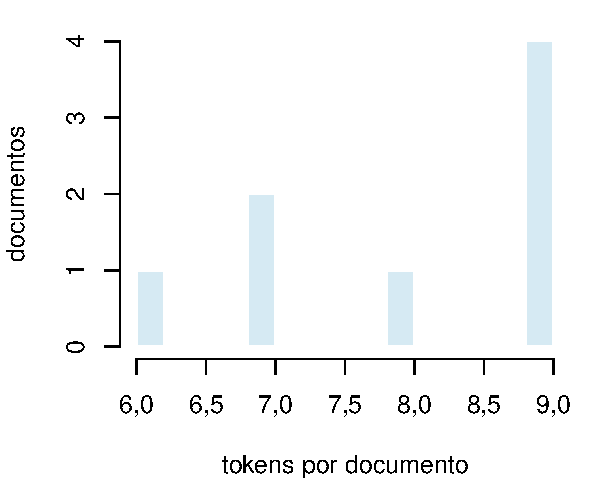
\includegraphics[width=0.52\linewidth]{figure/fig-tam-1} 

}


\end{knitrout}
  \fonte{Elaborada pelos autores.}
\end{figure}

\textbf{Os termos mais frequentes} são \texttt{de}, \texttt{a}, \texttt{documentos}, \texttt{e}, \texttt{busca}, \texttt{modelo}, \texttt{o}, \texttt{recuperacao}, \texttt{relevancia}, \texttt{acelera}. Diga quantos deles
dizem algo sobre o tema --- e o que isso sugere sobre as próximas aulas.

\textbf{Veredito.} Feche dizendo se o corpus responde às três perguntas da
Introdução. Se um descarte pegou, diga o que mudou no corpus por causa dele
--- um corpus corrigido por evidência vale mais do que um corpus que nunca foi
examinado.

O corpus é \textbf{provisório}: cresce na Aula 05, quando o grupo montar o
gabarito, e depois congela. Registre em uma frase o que as próximas aulas
podem mudar nele.

% ----------------------------------------------------------
% REFERÊNCIAS — não contam nas 3 páginas.
% Só aparecem as obras citadas. Para incluir uma obra não citada,
% use \nocite{chave}.
% ----------------------------------------------------------
\postextual
\bibliography{referencias}

\end{document}
